\documentclass[a4paper]{article}
\usepackage[utf8]{inputenc}
\usepackage{amsmath}
\usepackage{amssymb}
\usepackage{mathtools}
\usepackage{amsfonts}
\usepackage{lastpage}
\usepackage{pdfpages}
\usepackage{fancyvrb}
\usepackage[table]{colortbl}
\usepackage{fancyhdr}
\usepackage[linesnumbered, ruled]{algorithm2e}
\usepackage{graphicx}
\SetKwRepeat{Do}{do}{while}%
\usepackage[margin=2.5 cm]{geometry}


\pagestyle{fancy}
\cfoot{Page \thepage\ of \pageref{LastPage}}
\DeclareGraphicsExtensions{.pdf,.png,.jpg}
\author{Sigurdur Oli Arnason (5961181) \\ Victor Petren Bach Hansen (5990025)}
\title{Algorithms \& Networks \\ Exercise 4}
\lhead{Algorithms \& Networks}
\rhead{Exercise 4}

\begin{document}
\maketitle
\section{Counting numbers}
For $N=10000$, let $|P_k|$ denote the number of integers in the range $[1,2,\ldots,N]$ that $k$ divides. This number is equal to $\lfloor \frac{N}{k}\rfloor $. Let $|P_k \cap P_l|$ denote the number of integers in the range $[1,2,\ldots,N]$ that both $k$ and $l$ divides. This is equal to $\lfloor \frac{N}{k*l}\rfloor $. Using the inclusion/exclusion principle, we get that the number of integers, $D$, in the range $[1,2,\ldots, N]$ that is divisible by either 5, 11 or 19, is:
\begin{align*}
  D &=|P_5|+|P_{11}| + |P_{19}|-|P_{5}\cap P_{11}|-|P_{5}\cap P_{19}|-|P_{11}\cap P_{19}|+|P_{5}\cap P_{11} \cap P_{19} |\\
    &= 2000+909+564-181-105-47+9\\
    &= 3111
\end{align*}

\section{Inclusion/Exclusion for counting perfect matchings}
\subsection*{i)}
Since we in a perfect matching only have $n/2$ edges to cover all vertices $v\in V$, in order to satisfy the property that every $v$ must be incident to \textit{at least one} edge in $M$, each edge must be used to cover 2 unmatched vertices. If we don't it would mean that we e.g. used two edges to cover 3 vertices, resulting in 1 vertex being unmatched. Therefore, the number of perfect matchings is equal to the different number of ways we can chose a matching of size $n/2$, where each vertex has
to be incident to at least one edge.
\subsection*{ii)}
If we define the, for some $U \subseteq V $, the induced subgraph $G[U]=G'$, where $G'=(U,F)$, then this corresponds to the number of ways we can select $n/2$ different edges from $F$. We will call this number $N$ and the it has the formula
$$
  N=\binom{|F|}{n/2}
$$
This can easily be computed in polynomial time.
\subsection*{iii)}
We want to count the number of perfect matching some graph $G$ has. We know from $i)$ that this number is equal to the number of different ways we can arrange $n/2$ such that it satisfies the property that all vertices in $V$ are incident to at least one edge in the matching $M$. Surely, if we compute all the different ways we can choose $n/2$ edges from $G$, all perfect matches should be contained within these. However since we counted to many, we need to remove all non-perfect matches. If
we remove a vertex $v$ from $G$, ie $G[V\setminus \{v\}]$, the number of ways we can choose $n/2$ edges would all not be perfect matches, as this accounts for all the cases where $v$ is unmatched, so we can remove these. If we do this for each $v\in V$, we will count some cases twice (the cases where 2 vertices are unmatched), so we will have to add these again by counting the number of ways we can chose $n/2$ edges when removing all subsets of size 2. Continuing this approach, yields the
following inclusion/Exclusion formula:
$$
\sum_{X\subseteq V} (-1)^{|X|} N(G[V \setminus X])
$$
where the $X$ is all possible subsets of $V$ (incl the empty set) and the function $N$ is the result from $ii)$:
$$
N(G=(F,U)) = \binom{|F|}{n/2}
$$
\section{Sort and Search for exact satisfiability }
We split $X$ into $X_1 = \{x_1, x_2, ... ,x_{n/2}\}$ and $X_2 = \{x_{n/2+1}, ... ,x_{n}\}$. For every possible truth assignment
f of the variables of $X_1$ which assigns to each variable either the value true or false, we form its characteristic vector $V(f,X_1)$ where the i-th coordinate is equal to the number of literals which evaluate to true in the clause $c_i$. Do same for $X_2$.\\
We form two tables: Table $T_1$ contains characteristic vectors of $X_1$ and table $T_2$ contains characteristic vectors of $X_2$. Remove all vectors from the tables where $c_i > 1$ for any i. Sort the tables in order of how many clauses are true (now for exactly one literal).\\
Start with the value in $T_1$ with the lowest value and the largest one in $T_2$. Call the currently selected vectors in the tables $t_1$ and $t_2$ respectively. Define $|t|$ as the sum of it's values.\\
Repeat:\\
Move one value further in $T_1$ if $|t_1|+|t_2|<|C|$. \\
Move one value back in in $T_2$ if $|t_1|+|t_2|>|C|$. \\
If $|t_1|+|t_2|=|C|$:\\
\indent for all entries in $T_1$, $t_1'$, where $|t_1'| = |t_1|$\\
\indent \indent for all entries in $T_2$, $t_2'$, where $|t_2'| = |t_2|$\\
\indent \indent \indent if $t_1' + t_2'$ is true for exactly one literal in all clauses\\
\indent \indent \indent \indent return YES\\
\indent Move $T_1$ further until $|t_1|$ goes up.\\
\indent Move $T_2$ back until $|t_2|$ goes down.\\
If finished with $T_1$ and $T_2$\\
\indent return NO.\\
\\


\section{Maximum value matching and minimum cost flow}
As with the maximum matching in a bipartite graph approach, we transform $G$ into $G'$ by adding a source $s$ and a sink $t$ to the vertex set, and connect $s$ to all vertices in $V_1$ and $t$ to all vertices in $V_2$. We then assign a capacity of $1$ to all edges in the new graph $G'$. We also assign a cost to all outgoing edges of $s$ to $0$ and the same for all incoming edges of $t$. For all the edges $e$ that connects $V_1$ and $V_2$, we assign a cost of $-w(e)$.

Now the problem can be solved by finding a minimum cost flow from $s$ to $t$, which can be done using e.g. the cycle cancelling algorithms described in the lectures.
\section{Maximum size simple b-matching}
\subsection*{1}
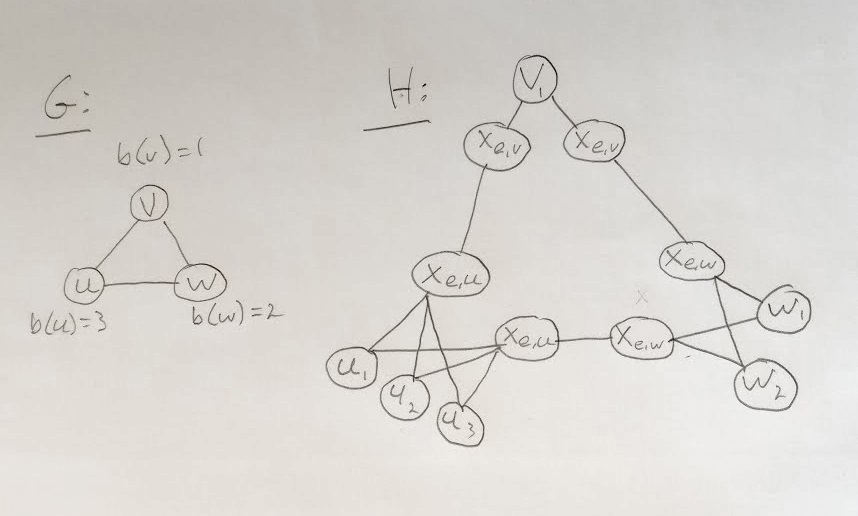
\includegraphics[width=\textwidth]{5}
\subsection*{2}
Say that $M_E$ is a b-matching with k edges for G. \\
For every edge $(u,v)$ in $M_E$ we pick edges $(u_i,x_{e,u})$ and $(v_j,x_{e,v})$ for some $i,j$ where $1<i<b(u)$ and $1<j<b(v)$. These are $2k$ such edges.\\
For all edges that are not in $M_E$ we pick edge $(x_{e,u},x_{e,v})$. There are $|E| - k$ such edges.\\
In total we then have $k+|E|$ edges and none of them share vertices so this is a matching for H.
\subsection*{3}

\subsection*{4}
In a maximum b-matching no vertex can be connected to more than $b(v)$ or $degree(v)$ vertices. So it does not change the solution to set the limit beforehand that $b'(v)=min\{b(v),degree(v)\}$.
\subsection*{5}
Find a maximum matching, $M_H$ in H in polynomial time. For each edge $(x_{e,u},x_{e,v})$ that is not in $M_H$ we choose edge $(u,v)$ in the matching for G, $M_G$. 
\subsection*{6}
Given $G=(V,E)$.\\
Set $B(v)=2$ for all vertices v in V.\\
Find maximum b-matching, M.\\
If all vertices in $(V,M)$ have degree 2 then YES. \\
If not NO.
\end{document}
